
\section{Independence of Vertical and Horizontal Motion}

Name \rule{2.0in}{0.1pt}\hfill{}Section \rule{1.0in}{0.1pt}\hfill{}Date \rule{1.0in}{0.1pt}

{\noindent \bf Objective:} \begin{list}{$\bullet$}{\itemsep0pt \parsep0pt}

\item Determine the relationship between vertical and horizontal motion

\end{list}

{\noindent \bf Apparatus:} \begin{list}{$\bullet$}{\itemsep0pt \parsep0pt}

\item two coins \item ruler

\end{list}

{\noindent \bf Activity:} \begin{enumerate}

\item Place a coin in the far corner of the table nearest the center aisle of the room. (See figure.) Lay a ruler next to the coin, parallel to the edge of the table along the aisle, allowing several centimeters at the end to hang over the far edge. Place a coin on the portion of the ruler hanging over the edge. Hold the ruler in place with a finger on the opposite end.

\vspace{0.3cm}
{\par\centering 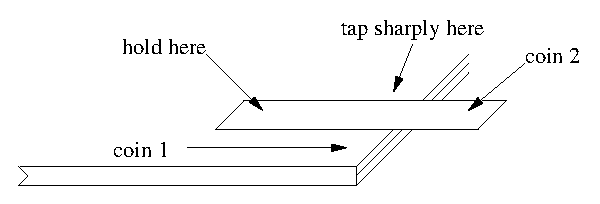
\includegraphics{independence_fig1.eps} \par}
\vspace{0.3cm}

\item With the ruler held, tap the side of the ruler opposite the coin sharply so that the coin on the table will be knocked over the edge of the table.

\item Both coins should land on the floor. Note, by sight or hearing, which hits the ground first.

\item Sketch the motion of the two coins.

\end{enumerate}

\vspace{40pt}

{\noindent \bf Questions:}

\begin{enumerate}
\item Which coin hit the floor first? Explain. \vspace{10mm}

\item What was the acceleration of each of the coins? Explain. \vspace{10mm}

\item Which coin had the greatest initial velocity? Explain. \vspace{10mm}

\item Which coin had the greatest final velocity? Explain
\end{enumerate}
